Given,
\begin{align}\label{eq:solutions/3/4/2/eq5}
\vec{x}^T\myvec{2 & \frac{-3}{2}\\\frac{-3}{2}& 4}\vec{x}+\myvec{ 10& -19}\vec{x}+23=0
\end{align}
The general second degree equation can be expressed as follows,
\begin{align}
\vec{x^T}\vec{V}\vec{x}+2\vec{u^T}\vec{x}+f=0\label{eq:solutions/3/4/2/eqmain}
\end{align}
From the given second degree equation we get,
\begin{align}
\vec{V} &= \myvec{2&\frac{-3}{2}\\\frac{-3}{2}&4}\\
\vec{u} &= \myvec{5\\\frac{-19}{2}}\\
f &= 23
\end{align}
Origin which is moved to the point is given by
$\vec{c}$
The above equation \eqref{eq:solutions/3/4/2/eqmain} can be modified as 
\begin{align}
(\vec{x}+\vec{c})^T\vec{V}(\vec{x}+\vec{c})+2\vec{u}^T(\vec{x}+\vec{c})+23&=0\label{eq:solutions/3/4/2/finalsub}
\end{align}
From equation \eqref{eq:solutions/3/4/2/finalsub} consider,
\begin{align}
    &\implies(\vec{x}+\vec{c})^T\vec{V}(\vec{x}+\vec{c})\\
    &\implies\vec{x}^T\vec{V}\vec{x}+\vec{c}^T\vec{V}\vec{x}+\vec{x}^T\vec{V}\vec{c}+\vec{c}^T\vec{V}\vec{c}\label{eq:solutions/3/4/2/1n}\\
    \intertext{we know that}
    &\vec{x}^T\vec{V}\vec{c}=\vec{c}^T\vec{V}\vec{x}\label{eq:solutions/3/4/2/p}
    \intertext{Substituting equation \eqref{eq:solutions/3/4/2/p} in equation \eqref{eq:solutions/3/4/2/1n}}
    &\implies\vec{x}^T\vec{V}\vec{x}+2\vec{c}^T\vec{V}\vec{x}+\vec{c}^T\vec{V}\vec{c}
%\label{eq:solutions/3/4/2/eq1}
\\
    \intertext{Equation \eqref{eq:solutions/3/4/2/finalsub} is modified as}
    &\implies\vec{x}^T\vec{V}\vec{x}+2\vec{c}^T\vec{V}\vec{x}+\vec{c}^T\vec{V}\vec{c}+2\vec{u}^T\vec{x}2\vec{u}^T\vec{c}+23=0
\end{align}
Equating \eqref{eq:solutions/3/4/2/finalsub} and  \eqref{eq:solutions/3/4/2/eq11}:
\begin{equation}\label{eq:solutions/3/4/2/eq1}
 \implies\vec{x}^T\vec{V}\vec{x}+2\vec{c}^T\vec{V}\vec{x}+\vec{c}^T\vec{V}\vec{c}+2\vec{u}^T\vec{x}2\vec{u}^T\vec{c}+23=
    \vec{x}^T\vec{V}\vec{x}-1
\end{equation}
From above equation \eqref{eq:solutions/3/4/2/eq1} we have,
\begin{align}\label{eq:solutions/3/4/2/eq2}
2\vec{c}^T\vec{V}\vec{x}+2\vec{u}^T\vec{x}=0
\end{align}
and
\begin{align}
2\vec{u}^T\vec{x}+\vec{v}^T\vec{c}=-22
\end{align}
From \eqref{eq:solutions/3/4/2/eq2}
\begin{align}
\vec{c}^T\vec{V}\vec{x}= -\vec{u}^T\vec{x}\\
\vec{c}^T\vec{V}= -\vec{u}^T\\
\vec{c}^T= -\vec{V}^{-1}\vec{u}^T \label{eq:solutions/3/4/2/eq45}
\end{align}
 Adjoining  $\vec V$ with identity matrix to compute inverse:
\begin{align}
\myvec{
2 &  \frac{-3}{2} &1 &0\\
 \frac{-3}{2} &4 & 0&1
}
  \xleftrightarrow[]{R_1 \leftarrow  \frac{1}{2}R_1}
\myvec{
1& \frac{-3}{4}&  \frac{1}{2}  &0\\
 \frac{-3}{2} &4 & 0 &1
}
\end{align}
\begin{align}
\myvec{
1& \frac{-3}{4}&  \frac{1}{2}  &0\\
 \frac{-3}{2} &4 & 0 &1
}
  \xleftrightarrow[]{R_2 \leftarrow R_2+\frac{3}{2} R_1}
\myvec{
1& \frac{-3}{4}& \frac{1}{2} &0\\
0 & \frac{23}{8} & \frac{3}{4} & 1}
\end{align}
\begin{align}
\myvec{
1& \frac{-3}{4}& \frac{1}{2} &0\\
0 & \frac{23}{8} & \frac{3}{4} & 1}
  \xleftrightarrow[]{R_2 \leftarrow\frac{8}{23}  R_2}
\myvec{
1& \frac{-3}{4}& \frac{1}{2} &0\\
0 & 1 & \frac{6}{23} &\frac{8}{23} }
\end{align}
\begin{align}
\myvec{
1& \frac{-3}{4}& \frac{1}{2} &0\\
0 & 1 & \frac{6}{23} &\frac{8}{23} }
  \xleftrightarrow[]{R_1 \leftarrow R_1+\frac{3}{4}R_2}
\myvec{
1& 0& \frac{16}{23} &\frac{6}{23}\\
0 & 1 & \frac{6}{23} &\frac{8}{23} }
\end{align}
\begin{align}
\vec V^{-1}=
\myvec{
\frac{16}{23} & \frac{6}{23}\\
\frac{6}{23}&\frac{8}{23}}
\end{align}
From \eqref{eq:solutions/3/4/2/eq45}
\begin{align}
\vec{c}^T=
\myvec{
\frac{-16}{23} &\frac{-6}{23}\\
\frac{-6}{23}& \frac{-8}{23}
}
\myvec{
5 \\\frac{-19}{2}
}
\end{align}
From above we have :
\begin{align}
 \vec{c}^T=
 \myvec{
 -1\\2
 }
\end{align}
Hence,
\begin{align}
 \vec c=
\myvec{
-1 &2}
\end{align}
From \eqref{eq:solutions/3/4/2/eq12} and \eqref{eq:solutions/3/4/2/eq11} when the origin is moved to the point  $\vec {c} = \myvec{-1 &2}$  $\vec{V}$ doesn't change
\begin{align}
    \det(\vec{V})&=5.75
\end{align}
Since $\det(\vec{V})>0$ the given equation represents the ellipse.
The characteristic equation of $\vec{V}$ is obtained by evaluating the determinant 
\begin{align}
       \begin{array}{|c|}
V-\lambda\vec{I}
\end{array}&=0\\
   \begin{array}{|cc|}
2-\lambda & \frac{-3}{2} \\ \frac{-3}{2} & 4-\lambda
\end{array}&=0\\
\implies 4\lambda^2-24\lambda+23&=0\label{eq:solutions/3/4/2/eqroots}
\end{align}
The eigenvalues are the roots of equation \ref{eq:solutions/3/4/2/eqroots} is given by 
\begin{align}
    \lambda_1&=\frac{6+\sqrt{13}}{2}\label{eq:solutions/3/4/2/eqeig1}\\
    \lambda_2&=\frac{6-\sqrt{13}}{2}\label{eq:solutions/3/4/2/eqeig2}
\end{align}
Hence from above:
\begin{align}\label{eq:solutions/3/4/2/d}
    \vec{D}=
    \myvec{
    \frac{6+\sqrt{13}}{2} & 0\\
     0 &\frac{6-\sqrt{13}}{2}
    }
\end{align}
The eigenvector $\vec{p}$ is defined as 
\begin{align}
    \vec{V}\vec{p}&=\lambda\vec{p}\\
    \implies (\vec{V}-\lambda\vec{I})\vec{p}&=0\label{eq:solutions/3/4/2/eqev}
\end{align}
For $\lambda_1=\frac{6+\sqrt{13}}{2}$ ,
\begin{align}
    (\vec{V}-\lambda_1\vec{I})=\myvec{\frac{-\sqrt{13}-2}{2} & \frac{-3}{2} \\\frac{-3}{2} & \frac{-\sqrt{13}+2}{2}}
\end{align}
\begin{align}
   \myvec{\frac{-\sqrt{13}-2}{2} & \frac{-3}{2} \\\frac{-3}{2} & \frac{-\sqrt{13}+2}{2}}
    \xleftrightarrow[]{R_1 \leftarrow R_1\div\frac{-\sqrt{13}-2}{2}}
    \myvec{
    1 &\frac{-\sqrt{13}-2}{2}\\
    \frac{-3}{2} & \frac{-\sqrt{13}-2}{2}
    }
\end{align}
\begin{align}
\myvec{
    1 &\frac{-\sqrt{13}-2}{2}\\
    \frac{-3}{2} & \frac{-\sqrt{13}-2}{2}
    }
    \xleftrightarrow[]{R_2 \leftarrow R_2\frac{-3}{2}R_1}
\myvec{
    1 &\frac{-\sqrt{13}-2}{2}\\
    0 &0
    }
    \end{align}
    \begin{align}\label{eq:solutions/3/4/2/p_1}
    \vec p_1=
    \myvec{
    \frac{-\sqrt{13}+2}{2}\\1
    }
\end{align}
For $\lambda_2=\frac{6-\sqrt{13}}{2}$ ,
\begin{align}
    (\vec{V}-\lambda_1\vec{I})=\myvec{\frac{\sqrt{13}-2}{2} & \frac{-3}{2} \\\frac{-3}{2} & \frac{\sqrt{13}+2}{2}}
\end{align}
\begin{align}
   \myvec{\frac{\sqrt{13}-2}{2} & \frac{-3}{2} \\\frac{-3}{2} & \frac{\sqrt{13}+2}{2}}
    \xleftrightarrow[]{R_1 \leftarrow R_1\div\frac{\sqrt{13}-2}{2}}
    \myvec{
    1 &\frac{-\sqrt{13}-2}{2}\\
    \frac{-3}{2} & \frac{-\sqrt{13}-2}{2}
    }
\end{align}
\begin{align}
\myvec{
    1 &\frac{-\sqrt{13}-2}{2}\\
    \frac{-3}{2} & \frac{-\sqrt{13}-2}{2}
    }
    \xleftrightarrow[]{R_2 \leftarrow R_2\frac{-3}{2}R_1}
\myvec{
    1 &\frac{-\sqrt{13}-2}{2}\\
    0 &0
    }
    \end{align}
    \begin{align}\label{eq:solutions/3/4/2/p_2}
    \vec p_2=
    \myvec{
    \frac{\sqrt{13}+2}{2}\\1
    }
    \end{align}
Again,for ellipse
\begin{align}
\vec{V}&=\vec{P}\vec{D}\vec{P^{-1}}
\intertext{Where $\vec{D}$ is a diagonal matrix, we get,}
\vec{P}&=\myvec{\vec{p_1}&\vec{p_2}}\\ \implies\vec{P}&=\myvec{\frac{-\sqrt{13}+2}{3} & \frac{\sqrt{13}+2}{3} \\1 & 1}\label{eq:solutions/3/4/2/eqP}\\
\vec{D}&=
    \myvec{
    \frac{6+\sqrt{13}}{2} & 0\\
     0 &\frac{6-\sqrt{13}}{2}
    }
\end{align}
Standard ellipse can be written in the form:
\begin{align}\label{eq:solutions/3/4/2/s}
    \vec{y}^T\vec{D}\vec{y}=\vec{u}^T\vec{V}^{-1}\vec{u}-f
\end{align}
Simplifying we get:
\begin{align}\label{eq:solutions/3/4/2/s1}
\vec{u}^T\vec{V}^{-1}\vec{u}=
\myvec{
5 &\frac{-19}{2}
}
\myvec
{
\frac{16}{23} & \frac{6}{23}\\
\frac{6}{23} & \frac{8}{23}
}
\myvec{
5\\\frac{-19}{2}
}
=24
\end{align}
substituting \eqref{eq:solutions/3/4/2/s1} in \eqref{eq:solutions/3/4/2/s} we have :
\begin{align}\label{eq:solutions/3/4/2/t}
 \vec{y}^T\vec{D}\vec{y}=1  
\end{align}
To get $\vec{y}$,
\begin{align}
\vec{y}&=\vec{P}^T\vec{x}-\vec{P}^T\vec{c}\\
    \vec{y}&=\myvec{\frac{-\sqrt{13}+2}{3} & 1 \\ \frac{\sqrt{13}+2}{3} & 1}
    \vec{x}-\myvec{\frac{-\sqrt{13}+2}{3} & 1\\ \frac{\sqrt{13}+2}{3} & 1}
\end{align}
Substituting  equation \eqref{eq:solutions/3/4/2/d}, in equation \eqref{eq:solutions/3/4/2/t} 
\begin{align}
    \vec{y}^T \myvec{
    \frac{6+\sqrt{13}}{2} & 0\\
     0 &\frac{6-\sqrt{13}}{2}
    }\vec{y}=1
\end{align}
\begin{figure}[h]
    \centering
    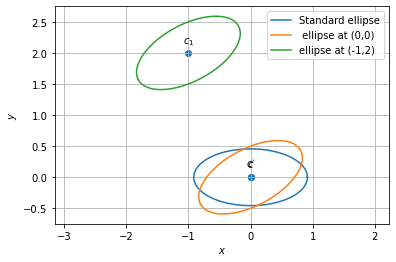
\includegraphics[width=\columnwidth]{./solutions/3/4/2/Assignment 6.png}
    \caption{Standard ellipse, Ellipse at (0,0) and  ellipse at (-1,2)}
    \label{eq:solutions/3/4/2/Fig :1}
\end{figure}

  


